\documentclass[../main.tex]{subfiles}
\graphicspath{{\subfix{../images/}}}
\begin{document}
\section{Parametric integration}
Just as we can differentiate parametrically, we can also evaluate definite integrals parametrically.

Suppose we want to evaluate the integral $\int_a^b y\,dx$ but we only know the parametric form $\begin{cases} x=x(t) \\ y=y(t) \end{cases}$ and eliminating the parameter is not feasible.

We just evaluate the values of $t$ when $x$ has the values $a$ and $b$, creating bounds for a new definite integral. We also change the function being integrated to $y(t)\times x'(t)$, then evaluate the definite integral.

E.g. Evaluate $\int_{-1}^{\frac{1}{2}}y\,dx$ for the parametric curve given by $\begin{cases} x=\sin{(t)} \\ y=2(\sin{(t)}+\cos{(t)}) \end{cases}$

First, we find $dx$:

$x=\sin{(t)}$

$dx=\cos{(t)}\,dt$

So now our integral is $\int \underbrace{2(\sin{(t)}+\cos{(t)})}_{y(t)}\underbrace{\cos{(t)}\,dt}_{dx}$

Next, we need to rewrite the upper and lower limits in terms of $t$:

Upper limit of integration:

$\sin{(t)}=\frac{1}{2}$

$t=\frac{\pi}{6}$

Lower limit:

$\sin{(t)}=-1$

$t=-\frac{\pi}{2}$

Our integral becomes $\int_{-\frac{\pi}{2}}^{\frac{\pi}{6}}2(\sin{(t)}+\cos{(t)})\cos{(t)}\,dt=\int_{-\frac{\pi}{2}}^{\frac{\pi}{6}}2\sin{(t)}\cos{(t)}+\cos^2{(t)}\,dt$

$\int_{-\frac{\pi}{2}}^{\frac{\pi}{6}}\sin{(2t)}+\cos{(2t)}+1\,dt$ (By the double-angle formulas)

$\Bigl[\frac{-\cos{(2t)}}{2}+\frac{\sin{(2t)}}{2}+t \Bigr]_{-\frac{\pi}{2}}^{\frac{\pi}{6}}$

$\Bigl(-\frac{1}{4}+\frac{\sqrt{3}}{2}+\frac{\pi}{6}\Bigr)-\Bigl(\frac{1}{2}+0-\frac{\pi}{2}\Bigr)=\frac{\sqrt{3}}{4}-\frac{3}{4}+\frac{2\pi}{3}$



\pagebreak

\subsection*{Questions}
(Answers - page \pageref*{Parametric integration answers})
\label{parametric integration}
\begin{enumerate}[itemsep=1cm]
    \item 
    Evaluate $\int_0^1 y\,dx$ for the parametric curve given by $\begin{cases} x=4-t \\ y=t^2-3t \end{cases}$

    \item 
    Evaluate $\int_{-\frac{1}{2}}^1 y\,dx$ for the parametric curve given by $\begin{cases} x=\sin{(t)} \\ y=2(\cos{(t)}-\sin{(t)}) \end{cases}$

    \item 
    Evaluate $\int_0^{\sqrt{3}}y\,dx$ for the parametric curve given by $\begin{cases} x=\tan{(t)} \\ y=\sin{(t)} \end{cases}$

    \item 
    Use parametric integration to show that the area of a circle of radius $r$ is $A=\pi r^2$, remembering that the parametric form of a circle is $\begin{cases} x=r\cos{(t)} \\ y=r\sin{(t)} \end{cases}$

    \item 
    Find the area enclosed between a parabola and its latus rectum, the line $x=a$, where $a>0$ and the parameterised equation for the parabola is $\begin{cases} x=at^2 \\ y=2at \end{cases}$

    \item 
    The graph shows the parametric function $\begin{cases} x=\cos{(2t)} \\ y=2(\cos{(t)}+\sin{(t)}) \end{cases} -\frac{\pi}{4}\leq t \leq \frac{3\pi}{4}$

    Find the area inside the curve.

    \begin{figure}[h]
       \centering
       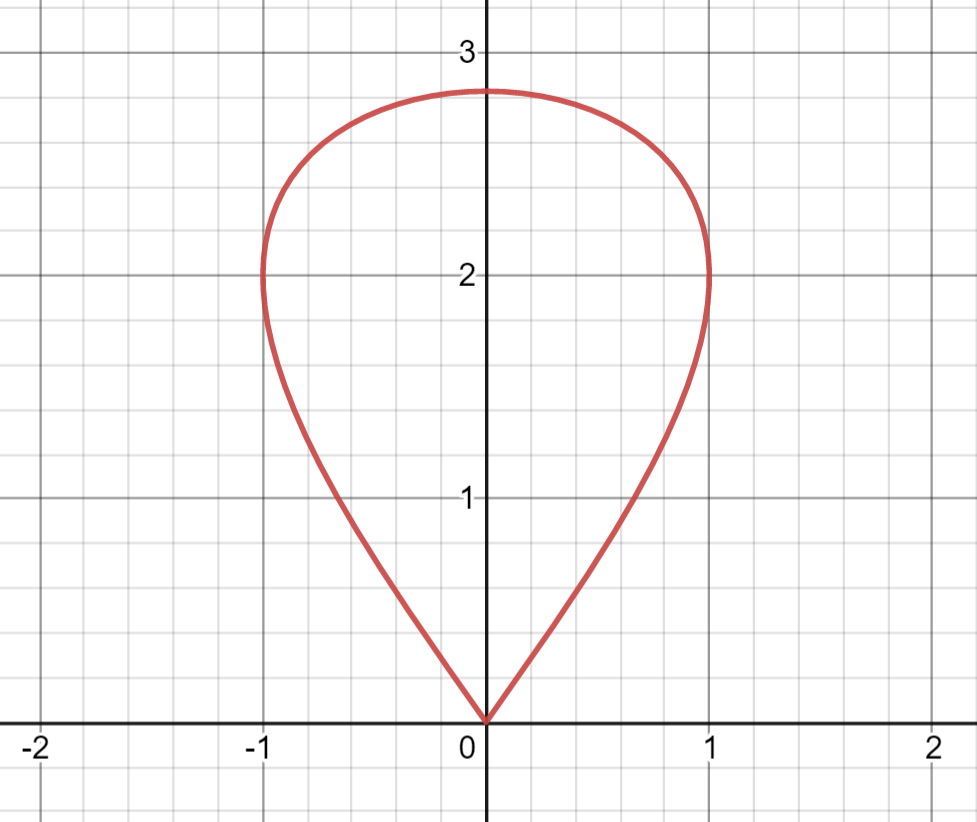
\includegraphics[width=0.3\linewidth]{images/parametricintegration.png}
    \end{figure}   

    \item 
    The astroid shown below is defined by the parametric equations 
    \[\begin{cases} x=\cos^3{(t)} \\ y=\sin^3{(t)} \end{cases} 0\leq t \leq 2\pi\]

    \begin{figure}[h]
        \centering
        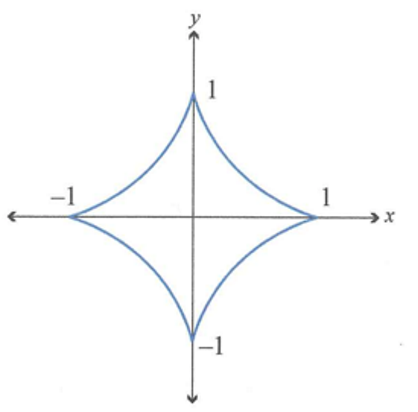
\includegraphics[width=0.3\linewidth]{images/parametricintegration2.png}
    \end{figure}

    By evaluating $\int_0^1 y\,dx$, or otherwise, calculate the exact area of the astroid.
\end{enumerate}
\pagebreak
\end{document}